\subsection{Цели и методика экспериментального исследования}
Целями экспериментального исследования было поставлено исследование:
\begin{itemize}
    \item Качество решений, предоставляемых алгоритмами.
    \item Временная сложность алгоритма.
\end{itemize}

Для проведения экспериментов было сгенерировано 3 набора данных:
\begin{enumerate}
    \item \label{item:known_opt_data} Набор данных с известных оптимумом, для постановки задачи с дополнительным ограничением $CR$
    \item Набор данных, основанных на слоистых графах, без известного оптимума, но с однородными процессорами. Данные из пункта \ref{item:known_opt_data} имеют свойство идеально сбалансированного разбиения, то есть разбиение от METIS всегда построит разбиение, близкое к разбиению идеального расписания. Чтобы проверить, как ведут себя алгоритмы на данных без такого свойства, были добавленно исследование на данных слоистых графов. Данный набор так же используется для исследований алгоритма для постановки задачи с дополнительным ограничением $CR$.
    \item Набор данных, основанный на слоистых графах, без исзвестного оптимума, но с неоднородными процессорами. Используется для постановки задачи без лополнительных ограничений
\end{enumerate}

Схема генерации слоистых графов описана в \cite{Canon_2019}.

\subsection{Экспериментальный стенд}

Эксперименты были проведены на машине, обладающей следующими характеристиками:
\begin{itemize}
    \item CPU Intel Xeon E5-2605 v4, 2.2Ггц
    \item 62Гб оперативной памяти
\end{itemize}

\subsection{Исследование качества решений}

\subsubsection{Жадный алгоритм с жадным критерием}

\paragraph{Постановка CR}

\begin{figure}[!htbp]
    \centering
    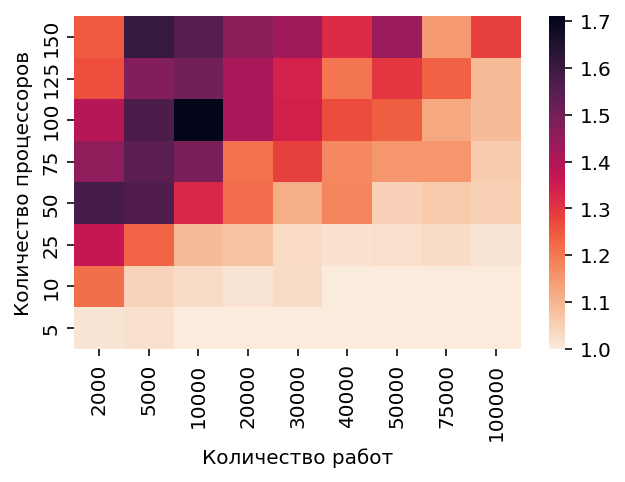
\includegraphics[width=\textwidth]{imgs/ideal_1/CR/th.png}
    \caption{Отношение времени выполнения расписания к оптимальному времени выполнения (тепловая карта)}
    \label{fig:CR-GC1-times-heatmap}
\end{figure}

\begin{figure}[!htbp]
    \centering
    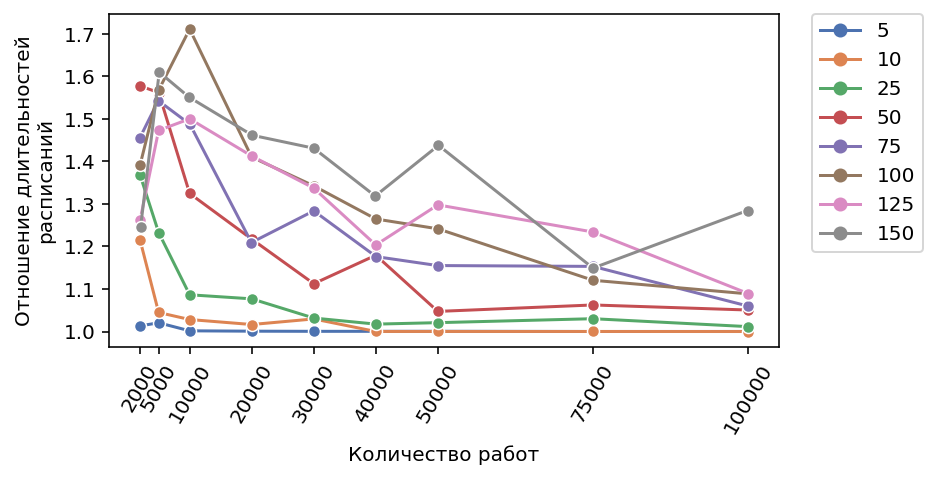
\includegraphics[width=\textwidth]{imgs/ideal_1/CR/gr_amalgamated.png}
    \caption{Отношение времени выполнения расписания к оптимальному времени выполнения}   
    \label{fig:CR-GC1-times-compiled} 
\end{figure}

На рисунках \ref{fig:CR-GC1-times-heatmap} и \ref{fig:CR-GC1-times-compiled} показано качество решенией, генерируемых жадных алгоритмом с жадными критерием на данных с известным оптимумом. Цветом на рисунке \ref{fig:CR-GC1-times-heatmap} и значением на оси $Oy$ на рисунке \ref{fig:CR-GC1-times-compiled} показано отношение длительности расписания, построенного алгоритмом к длительности оптимального расписания. Значения всегда больше 1, чем меньше, тем лучше.

Точность алгоитма повышается с увеличением количества работа и уменьшается с повышением количества процессоров в системе. 

\begin{figure}[!htbp]
    \centering
    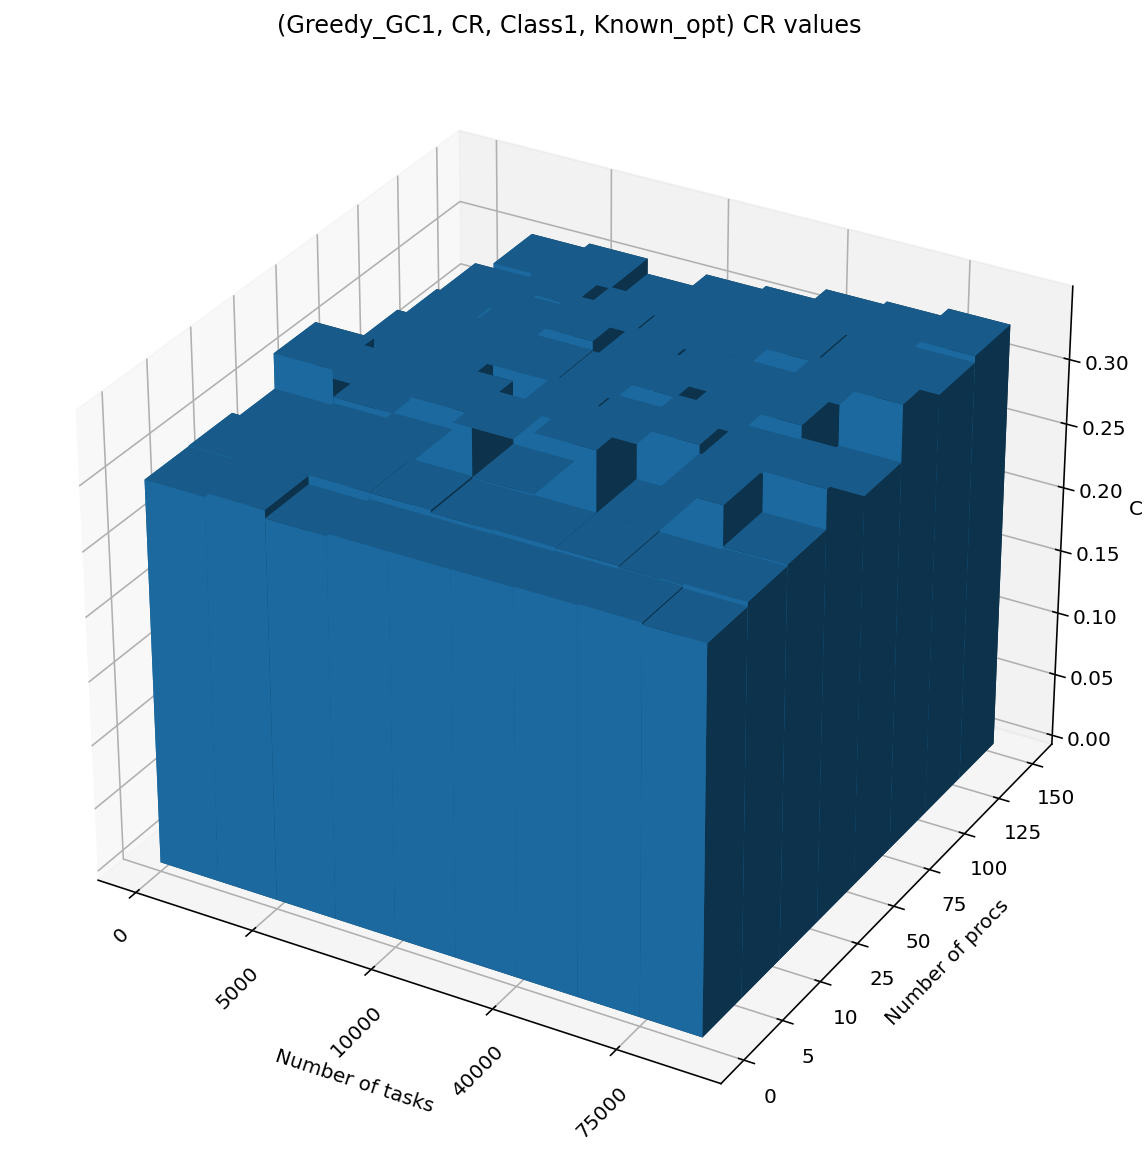
\includegraphics[width=\textwidth]{imgs/ideal_1/CR/cr_3d.png}
    \caption{12345}
\end{figure}

\begin{figure}[!htbp]
    \centering
    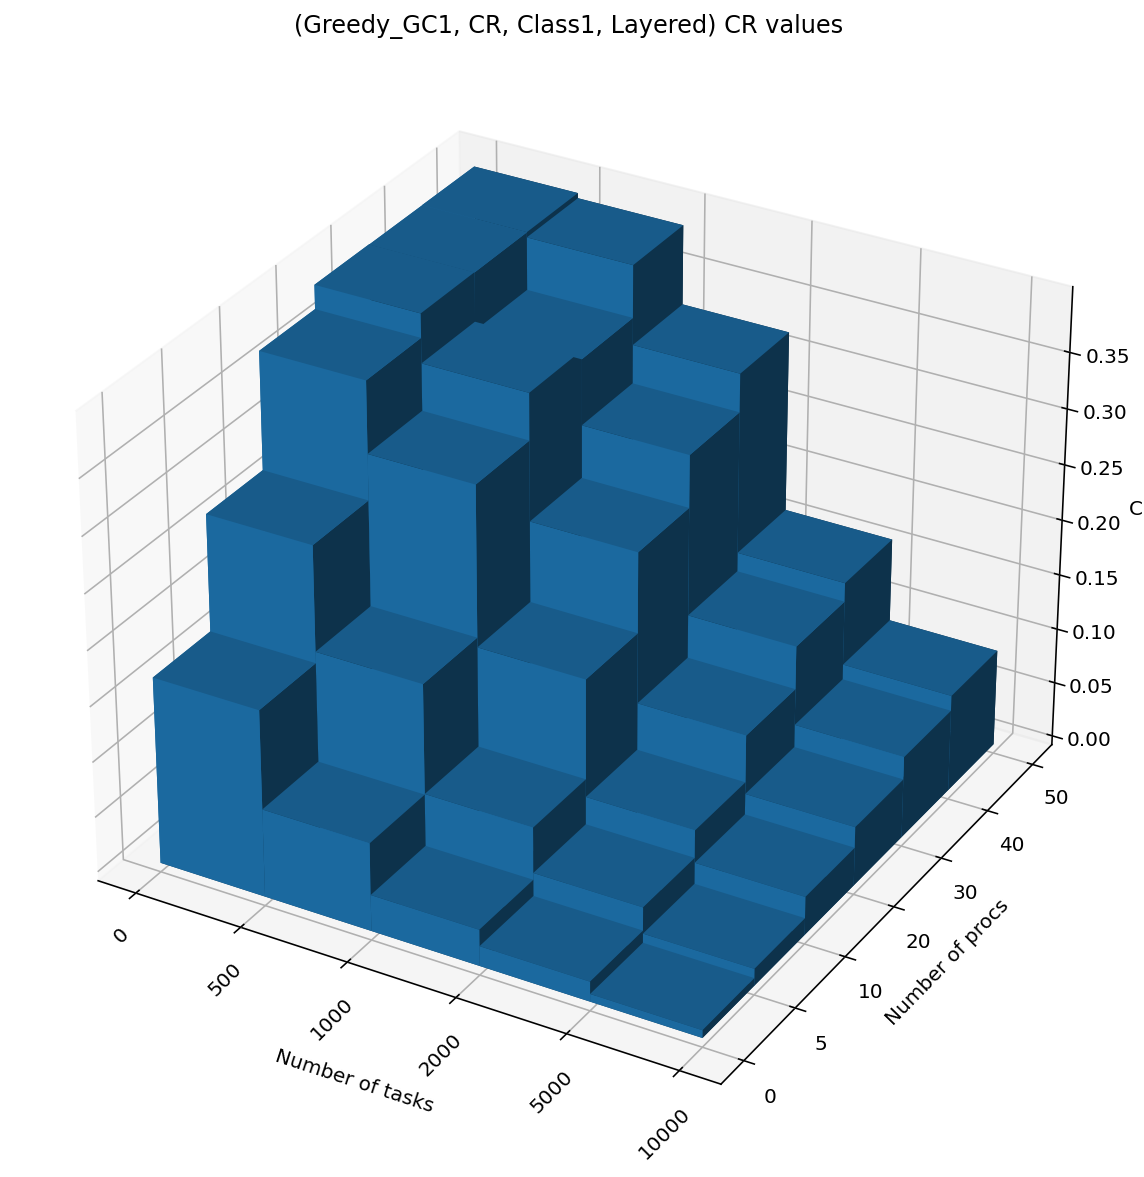
\includegraphics[width=\textwidth]{imgs/layered_class_1/CR/cr_3d.png}
    \caption{12345}    
\end{figure}

\subsubsection{Жадный алгоритм с EDF эвристикой}

\paragraph{Постановка CR}

\begin{figure}[!htbp]
    \centering
    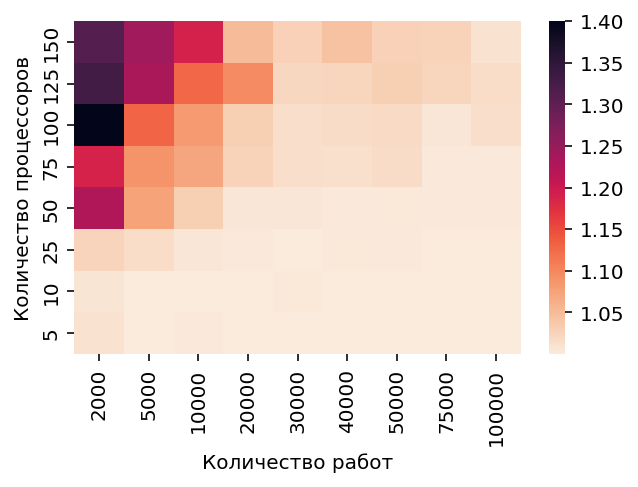
\includegraphics[width=\textwidth]{imgs/ideal_1/CR_EDF/th.png}
    \caption{Отношение времени выполнения расписания к оптимальному времени выполнения (тепловая карта)}
    \label{fig:CR-EDF-times-heatmap}
\end{figure}

\begin{figure}[!htbp]
    \centering
    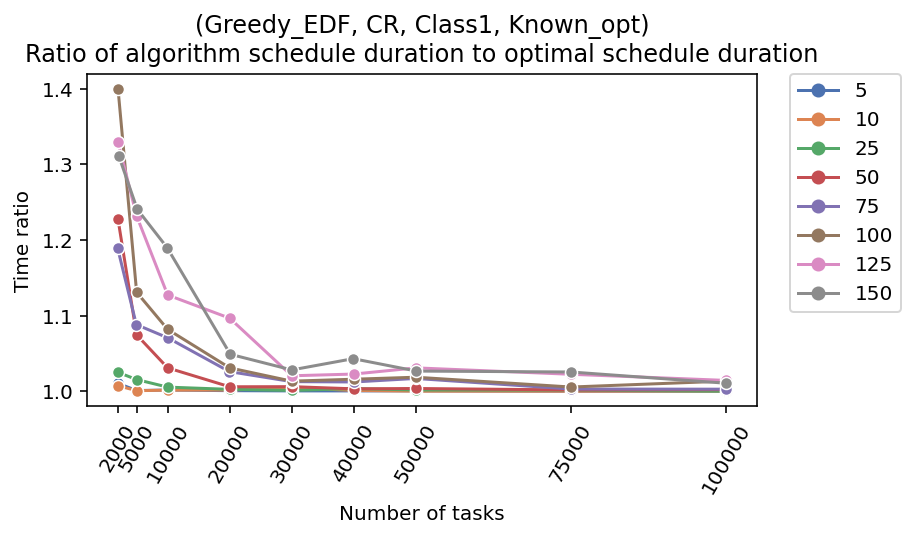
\includegraphics[width=\textwidth]{imgs/ideal_1/CR_EDF/gr_amalgamated.png}
    \caption{Отношение времени выполнения расписания к оптимальному времени выполнения} 
    \label{fig:CR-EDF-times-compiled}
\end{figure}

На рисунках \ref{fig:CR-EDF-times-heatmap} и \ref{fig:CR-EDF-times-compiled} показано качество решенией, генерируемых жадным алгоритмом с жадными критерием на данных с известным оптимумом. Цветом на рисунке \ref{fig:CR-EDF-times-heatmap} и значением на оси $Oy$ на рисунке \ref{fig:CR-EDF-times-compiled} показано отношение длительности расписания, построенного алгоритмом к длительности оптимального расписания. Значения всегда больше 1, чем меньше, тем лучше.

Точность алгоритма повышается с увеличением количества работ, однако ухудшение решения с увеличением количества процессоров в системе менее значительно, чем в жадном алгоритме с жадным критерием. 

\begin{figure}[!htbp]
    \centering
    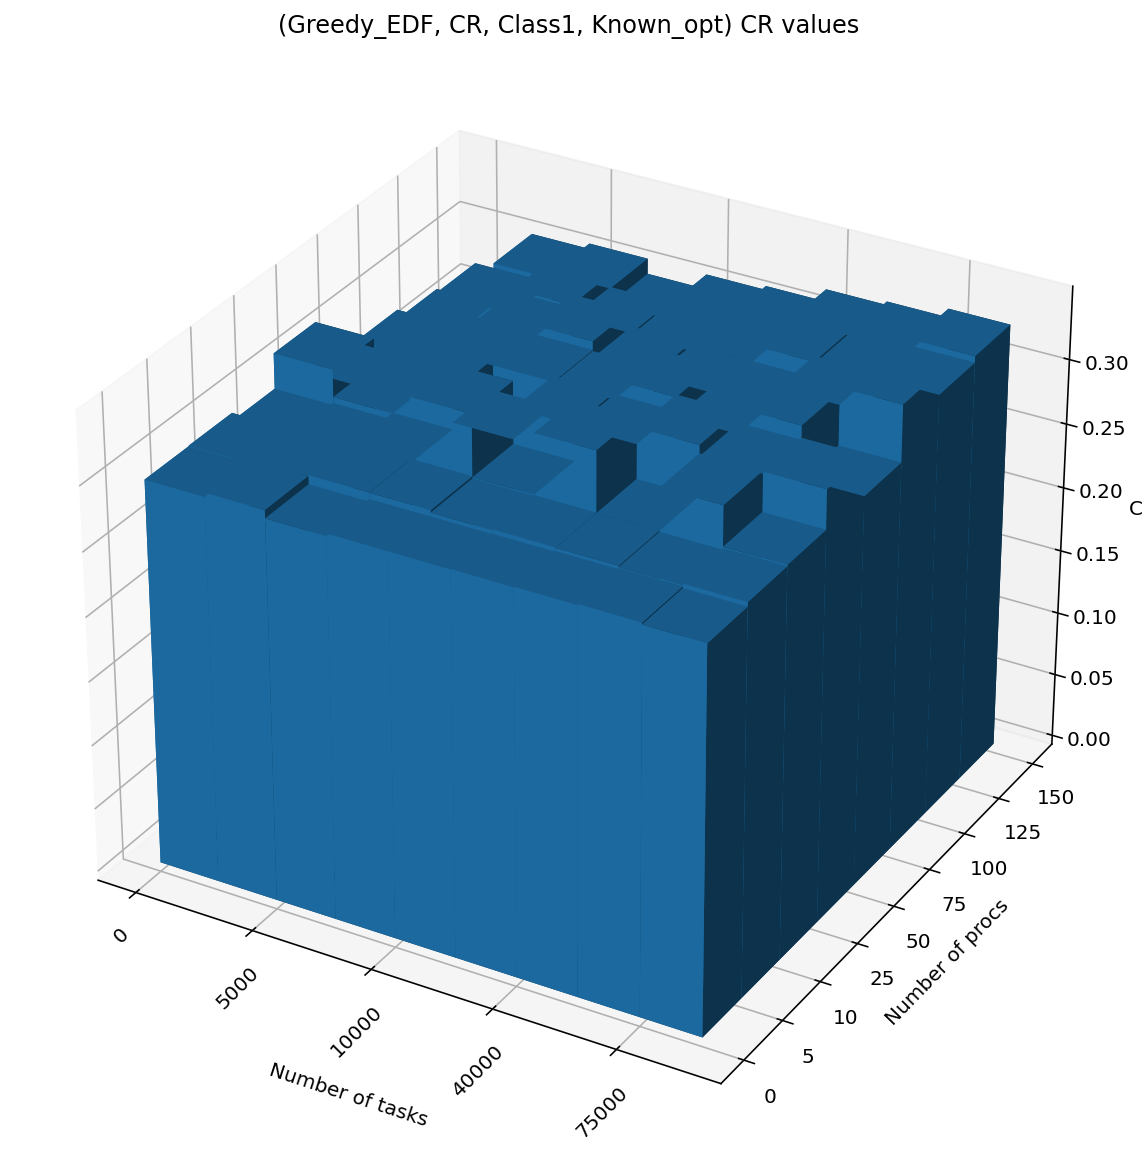
\includegraphics[width=\textwidth]{imgs/ideal_1/CR_EDF/cr_3d.png}
    \caption{12345}
\end{figure}

\begin{figure}
    \centering
    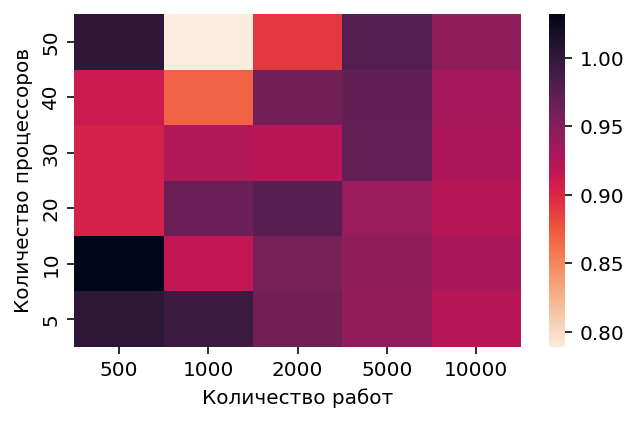
\includegraphics[width=\textwidth]{imgs/layered_class_1/CR_EDF/times.png}
    \caption{Отношение времени выполнения расписания к времени выполнения расписания, построенного при помощи жадного алгоритма с жадным критерием (тепловая карта)}
    \label{fig:CR-layered-EDF-times-heatmap}
\end{figure}

\begin{figure}[!htbp]
    \centering
    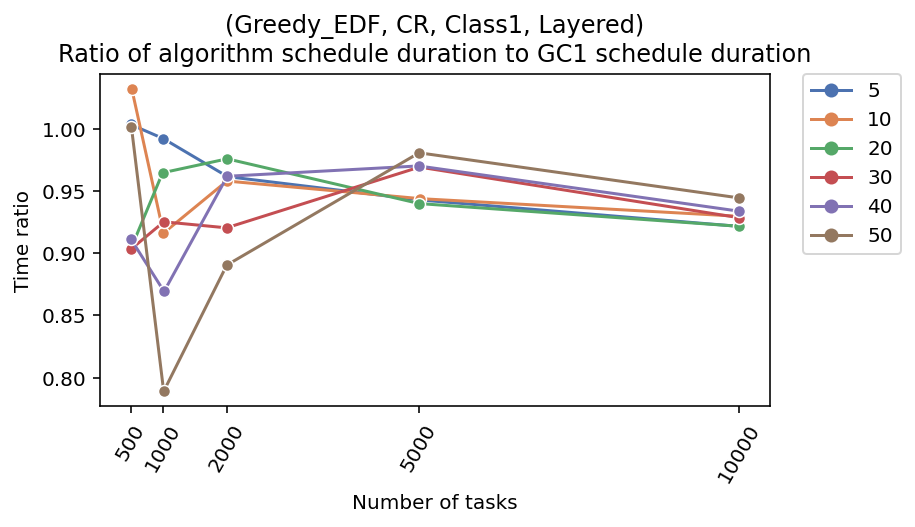
\includegraphics[width=\textwidth]{imgs/layered_class_1/CR_EDF/gr_amalgamated.png}
    \caption{Отношение времени выполнения расписания к времени выполнения расписания, построенного при помощи жадного алгоритма с жадным критерием}
    \label{fig:CR-layered-EDF-times-compiled}
\end{figure}

На рисунках \ref{fig:CR-layered-EDF-times-heatmap} и \ref{fig:CR-layered-EDF-times-compiled} показано качество решений, генерируемых жадным алгоритмом с EDF эвристикой на данных, построенных на слоистых графах. Цветом на рисунке \ref{fig:CR-layered-EDF-times-heatmap} и значением на оси $Oy$ на рисунке \ref{fig:CR-layered-EDF-times-compiled} показано отношение длительности расписании расписании, построенного жадным алгоритмом с жадным кртерием. Значения всегда больше 1, чем меньше, тем лучше.

В большинстве случаев, качество решений жадного алгоритма с EDF эвристикой лучше качества решений жадного лагоритма с жадным критерием, однако преимущество остается в пределах 10\%, кроме двух выбросов в районе 1000 работ. 

\begin{figure}[!htbp]
    \centering
    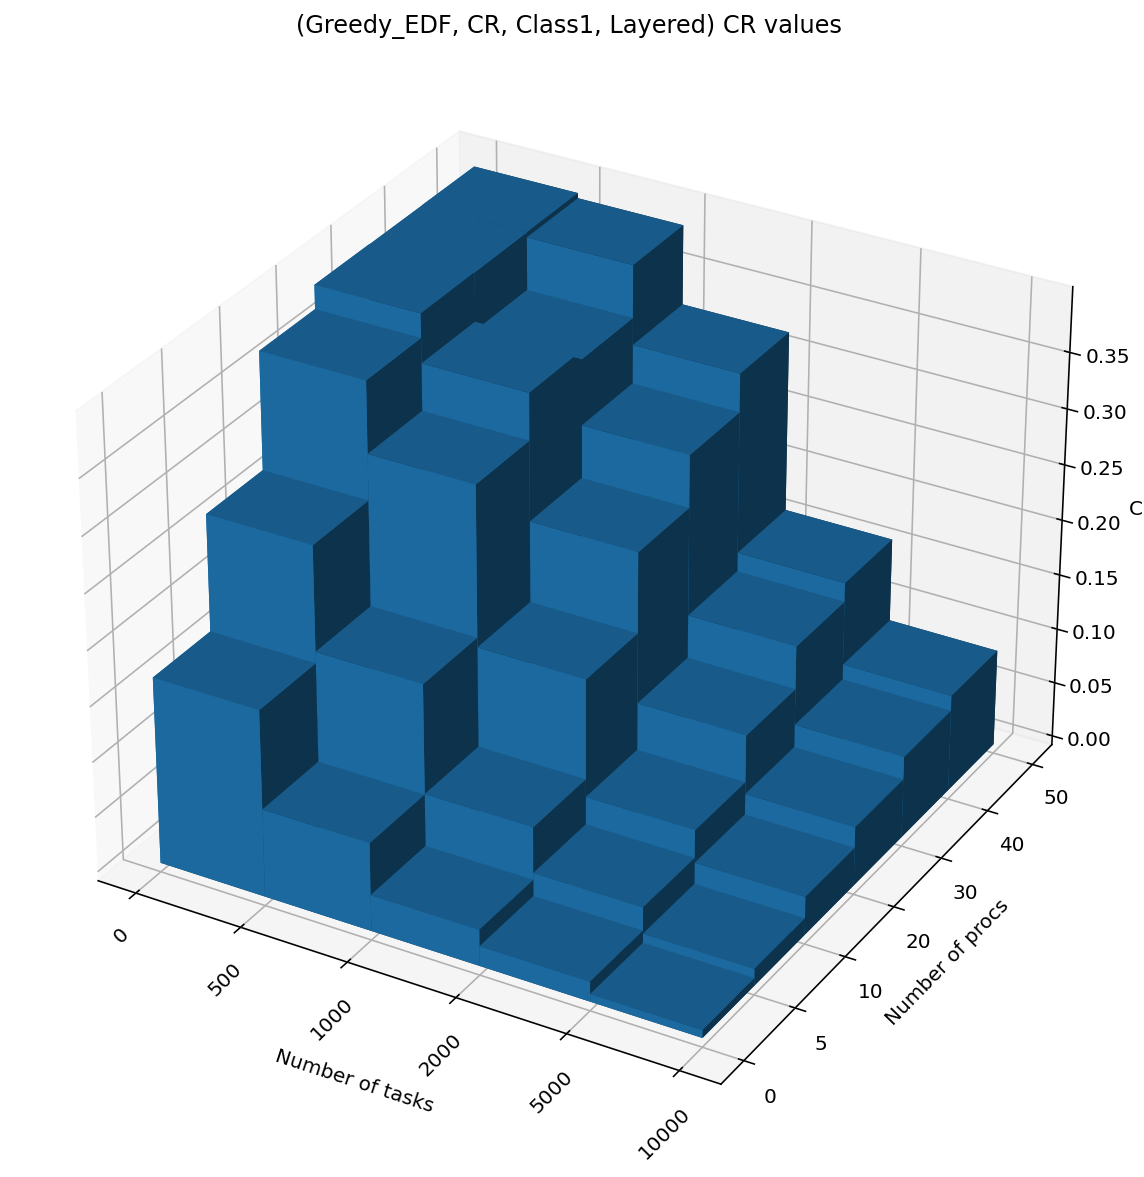
\includegraphics[width=\textwidth]{imgs/layered_class_1/CR_EDF/cr_3d.png}
    \caption{12345}
\end{figure}

\paragraph{Постановка NO}

\begin{figure}[!htbp]
    \centering
    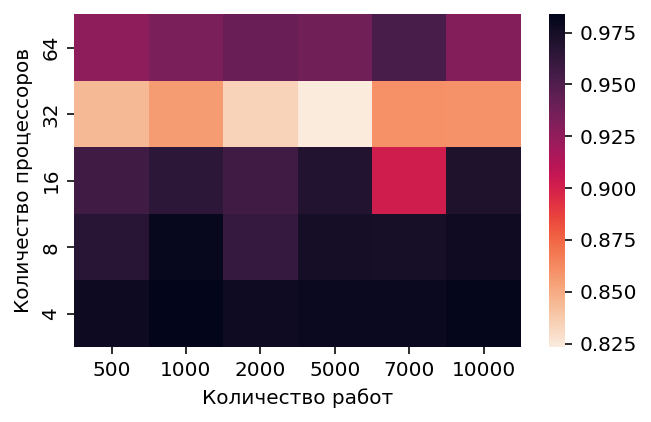
\includegraphics[width=\textwidth]{imgs/unbalanced/NO_EDF/times.png}
    \caption{Отношение времени выполнения расписания к времени выполнения расписания, построенного при помощи жадного алгоритма с жадным критерием (тепловая карта)}
    \label{fig:NO-EDF-times-heatmap}
\end{figure}

\begin{figure}[!htbp]
    \centering
    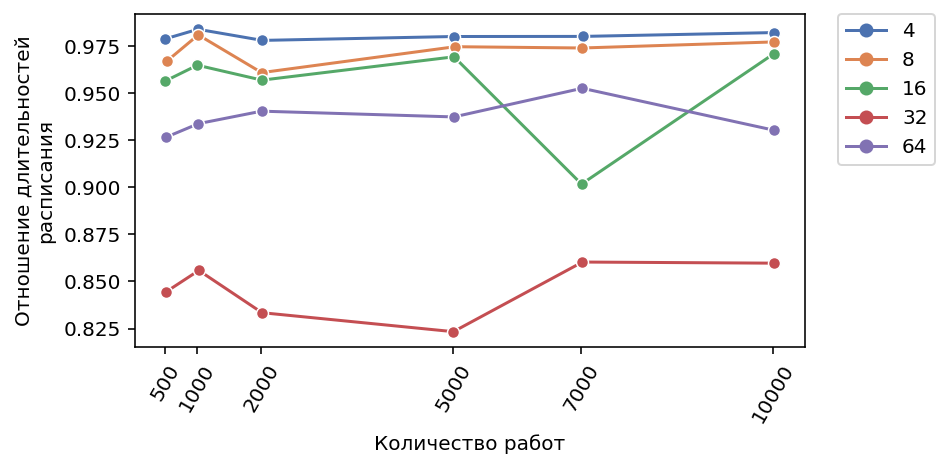
\includegraphics[width=\textwidth]{imgs/unbalanced/NO_EDF/gr_amalgamated.png}
    \caption{Отношение времени выполнения расписания к времени выполнения расписания, построенного при помощи жадного алгоритма с жадным критерием}
    \label{fig:NO-EDF-times-compiled}
\end{figure}

На рисунках \ref{fig:NO-EDF-times-heatmap} и \ref{fig:NO-EDF-times-compiled} показано качество решений, генерируемых жадным алгоритмом с EDF эвристикой на данных, построенных на слоистых графах. Цветом на рисунке \ref{fig:NO-EDF-times-heatmap} и значением на оси $Oy$ на рисунке \ref{fig:NO-EDF-times-compiled} показано отношение длительности расписании расписании, построенного жадным алгоритмом с жадным кртерием. Значения всегда больше 1, чем меньше, тем лучше.

Во всех случаях, качество решений выше качетва решений жадного алгоритма с жадным критерием, но это улучшение не превышает 10\%, за исключением случая с 32 процессорами.

\subsection{Исследование временной сложности алгоритма}

\subsubsection{Жадный алгоритм с жадным критерием}

\paragraph{Постановка CR}

\begin{figure}[!htbp]
    \centering
    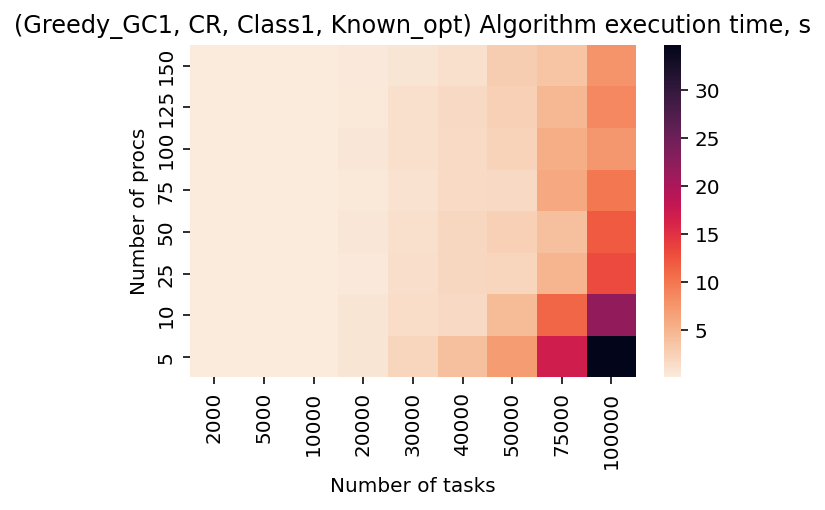
\includegraphics[width=\textwidth]{imgs/ideal_1/CR/et_heatmap.png}
    \caption{Время выполнения алгоритма, в секундах (тепловая карта)}
    \label{fig:CR-exec-time-heatmap}
\end{figure}

\begin{figure}[!htbp]
    \centering
    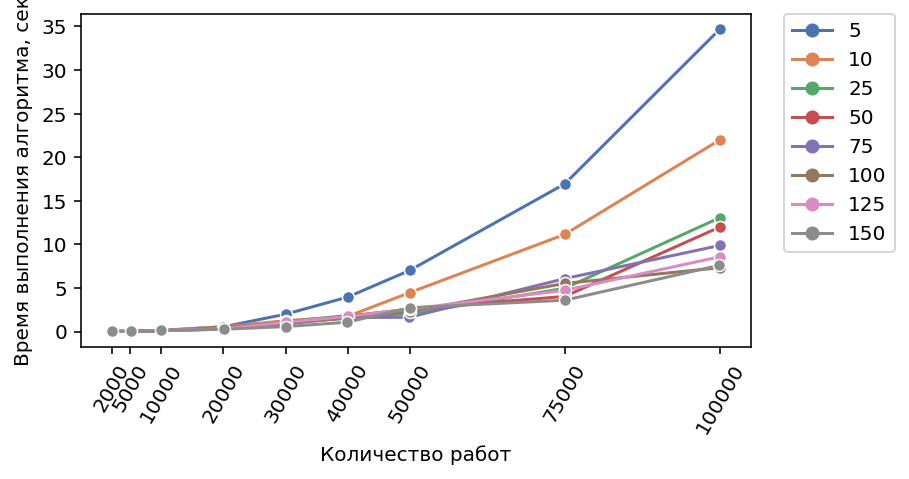
\includegraphics[width=\textwidth]{imgs/ideal_1/CR/tr_graph.png}
    \caption{Время выполнения алгоритма, в секундах}
    \label{fig:CR-exec-time-compiled}
\end{figure}

На рисунках \ref{fig:CR-exec-time-heatmap} и \ref{fig:CR-exec-time-compiled} показано время выполнения жадного алгоритма с жадным критерием, включая прогоны METIS. Время выполнения растет с увеличением количества вершин. При равном количестве работ, выше время выполнения при меньшем количестве процессоров. Причина в том, что при равном количестве работ и понижении количества процессоров повышается количество работ, распределенных на процессор, что приводит к большему количеству пропусков в расписании, что значит, что алгоритм постановки работы в расписании отработает быстрее, т.к. он работает до первого найденного доступного простоя на процессоре. 

\begin{figure}[!htbp]
    \centering
    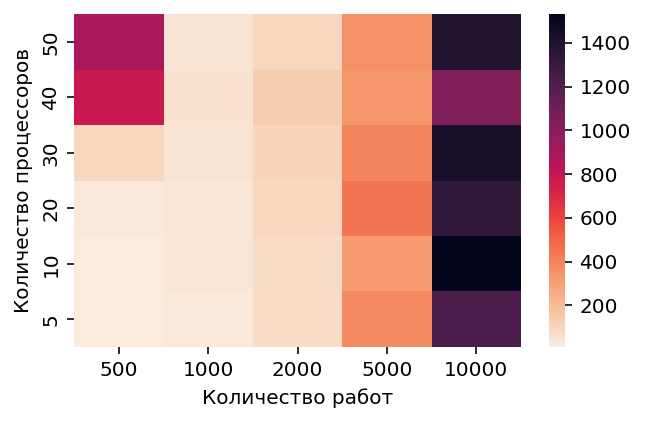
\includegraphics[width=\textwidth]{imgs/layered_class_1/CR/et_heatmap.png}
    \caption{Время выполнения алгоритма, в миллисекундах (тепловая карта)}
    \label{fig:CR-layered-exec-time-heatmap}
\end{figure}

\begin{figure}[!htbp]
    \centering
    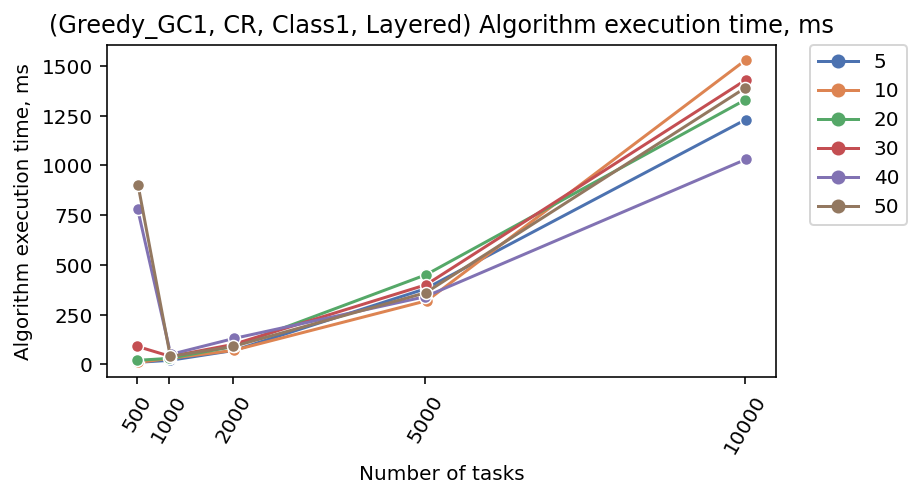
\includegraphics[width=\textwidth]{imgs/layered_class_1/CR/tr_graph.png}
    \caption{Время выполнения алгоритма, в миллисекундах}
    \label{fig:CR-layered-exec-time-compiled}
\end{figure}

На рисунках \ref{fig:CR-layered-exec-time-heatmap} и \ref{fig:CR-layered-exec-time-compiled} показано время выполнения алгоритма на наборе данных, основанных на слоистых графах. Кроме двух выбросов, соотносящихся с самым малым количеством работ и самым большим количеством процессоров в системе, нет существенной зависимости времени выполнения от количества процессоров в системе.

\paragraph{Постановка NO}

\begin{figure}[!htbp]
    \centering
    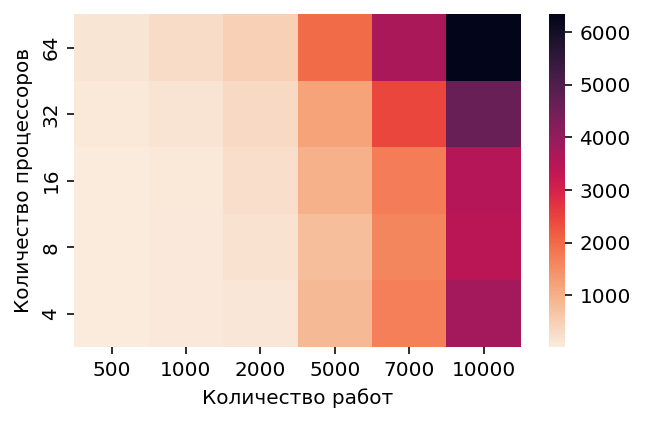
\includegraphics[width=\textwidth]{imgs/unbalanced/NO/et_heatmap.png}
    \caption{Время выполнения алгоритма, в миллисекундах (тепловая карта)}
    \label{fig:NO-exec-time-heatmap}
\end{figure}

\begin{figure}[!htbp]
    \centering
    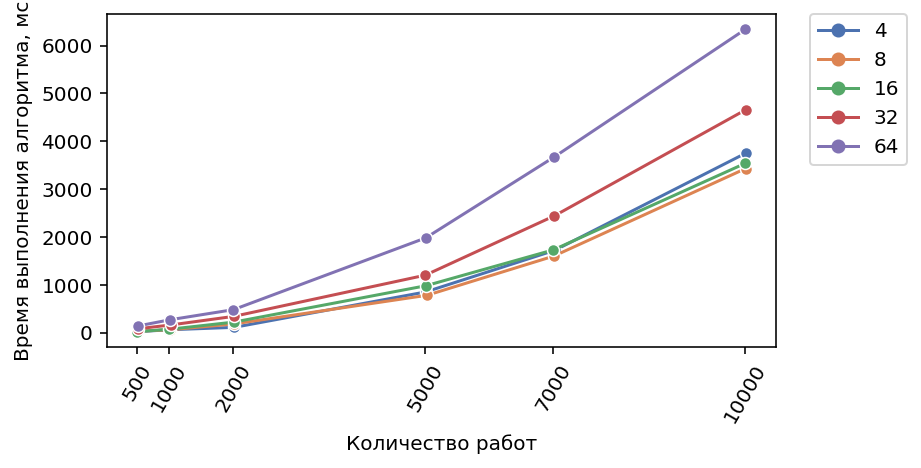
\includegraphics[width=\textwidth]{imgs/unbalanced/NO/tr_graph.png}
    \caption{Время выполнения алгоритма, в миллисекундах}
    \label{fig:NO-exec-time-compiled}
\end{figure}

На рисунках \ref{fig:NO-exec-time-heatmap} и \ref{fig:NO-exec-time-compiled} показано время выполнения алгоритма на наборе данных c неоднородными процессорами. Время выполнения увеличивается с увеличением количества задач и с увеличением количества процессоров.

\subsubsection{Жадный алгоритм с EDF эвристикой}

\paragraph{Постановка CR}

\begin{figure}[!htbp]
    \centering
    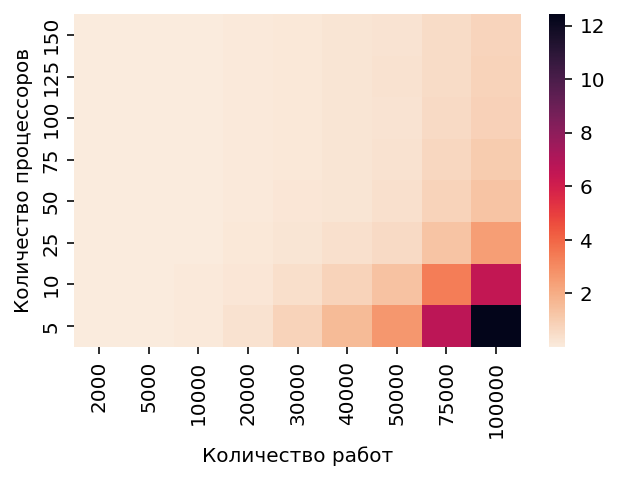
\includegraphics[width=\textwidth]{imgs/ideal_1/CR_EDF/et_heatmap.png}
    \caption{Время выполнения алгоритма, в секундах (тепловая карта)}
    \label{fig:CR-EDF-exec-time-heatmap}
\end{figure}

\begin{figure}[!htbp]
    \centering
    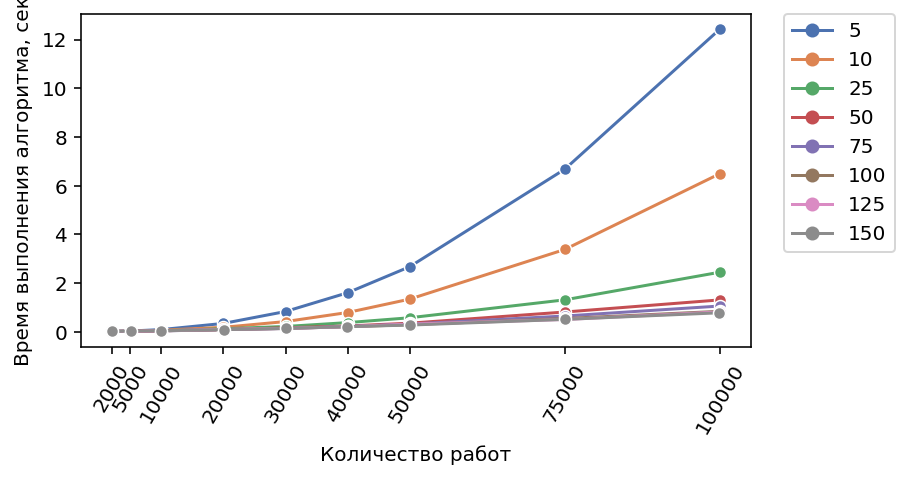
\includegraphics[width=\textwidth]{imgs/ideal_1/CR_EDF/tr_graph.png}
    \caption{Время выполнения алгоритма, в секундах}
    \label{fig:CR-EDF-exec-time-compiled}
\end{figure}

На рисунках \ref{fig:CR-EDF-exec-time-heatmap} и \ref{fig:CR-EDF-exec-time-compiled} показано время выполнения жадного алгоритма с EDF эвристикой, включая прогоны METIS. Время выполнения растет с увеличением количества вершин, при этом в несколько раз меньшим времени, затраченного на прогон жадного алгоритма с жадным критерием. При равном количестве работ, выше время выполнения при меньшем количестве процессоров. Причина схожа с причинами подобного явления для жадного алгоритма с жадным критерием, поскольку они разделяют одну процедуру поиска нового места в распсиании. 

\begin{figure}[!htbp]
    \centering
    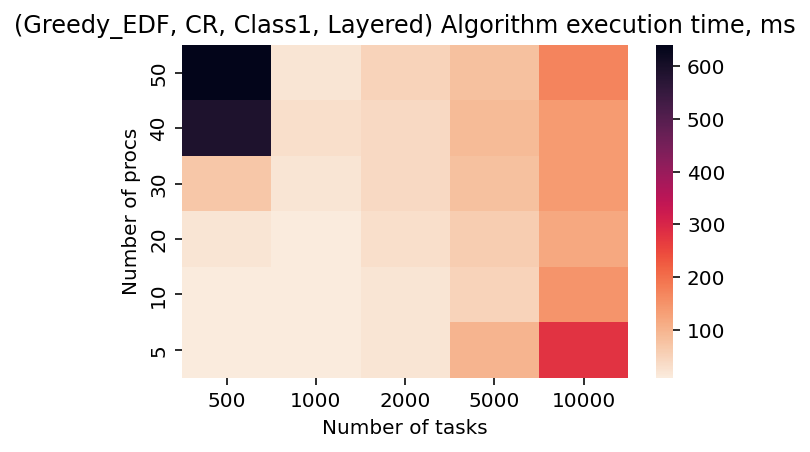
\includegraphics[width=\textwidth]{imgs/layered_class_1/CR_EDF/et_heatmap.png}
    \caption{Время выполнения алгоритма, в миллисекундах (тепловая карта)}
    \label{fig:CR-layered-EDF-exec-time-heatmap}
\end{figure}

\begin{figure}[!htbp]
    \centering
    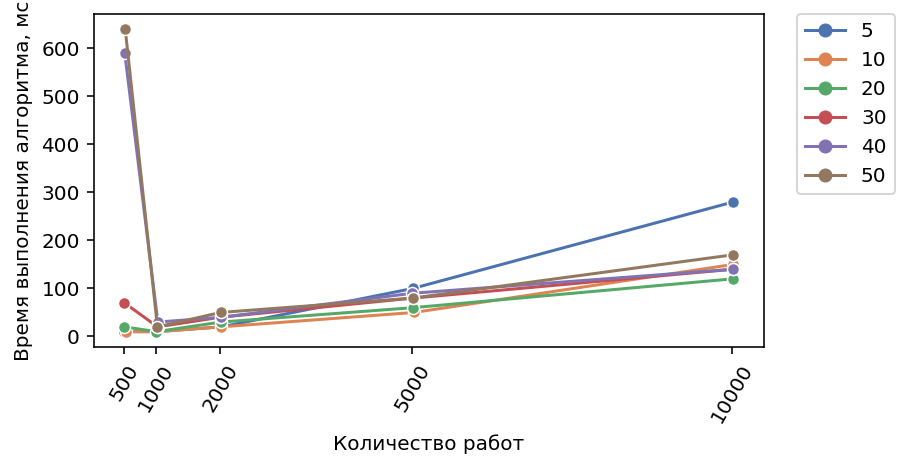
\includegraphics[width=\textwidth]{imgs/layered_class_1/CR_EDF/tr_graph.png}
    \caption{Время выполнения алгоритма, в миллисекундах}
    \label{fig:CR-layered-EDF-exec-time-compiled}
\end{figure}

На рисунках \ref{fig:CR-layered-EDF-exec-time-heatmap} и \ref{fig:CR-layered-EDF-exec-time-compiled} показано время выполнения жадного алгоритма с EDF эвристикой, включая прогоны METIS, на слоистых данных, основанных на слоистых графах. Как и для жадного алгоритма с жадной эвристикой, на данных видно два выброса, которые соотносятся с самым большим количеством процессором и самым маленьким количеством работ в исходных данных. Также не существует значимой зависимости между количеством процессоров в системе и временем, затраченным на построение расписания. Алгоритм работает в несколько раз быстрее жадного алгоритма с жадным критерием.

\paragraph{Постановка NO}

\begin{figure}[!htbp]
    \centering
    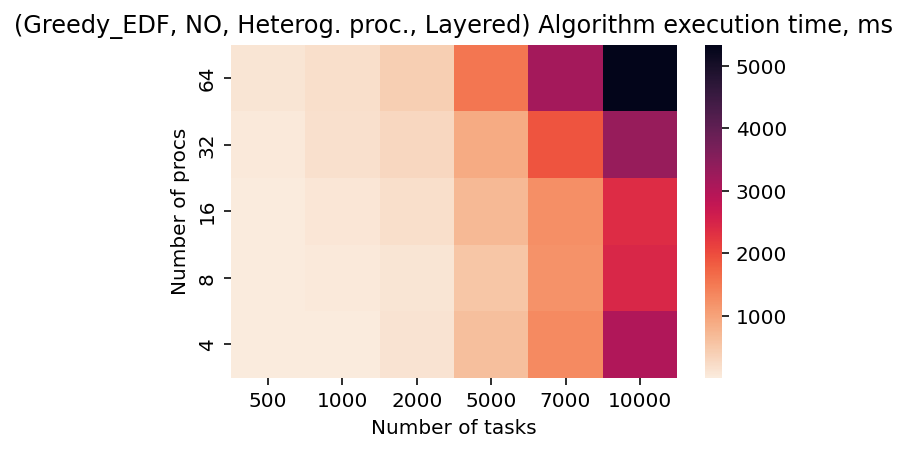
\includegraphics[width=\textwidth]{imgs/unbalanced/NO_EDF/et_heatmap.png}
    \caption{Время выполнения алгоритма, в миллисекундах (тепловая карта)}
    \label{fig:NO-EDF-exec-time-heatmap}
\end{figure}

\begin{figure}[!htbp]
    \centering
    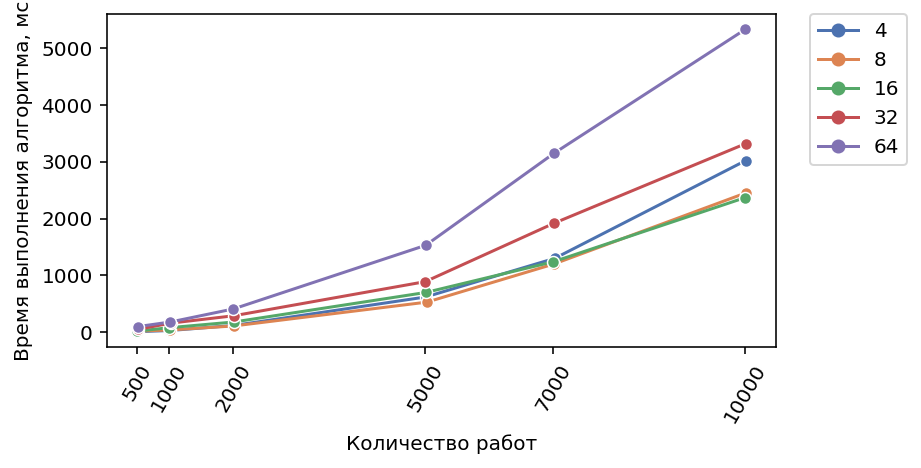
\includegraphics[width=\textwidth]{imgs/unbalanced/NO_EDF/tr_graph.png}
    \caption{Время выполнения алгоритма, в миллисекундах}
    \label{fig:NO-EDF-exec-time-compiled}
\end{figure}

На рисунках \ref{fig:CR-layered-EDF-exec-time-heatmap} и \ref{fig:CR-layered-EDF-exec-time-compiled} показано время выполнения жадного алгоритма с EDF эвристикой, включая прогоны METIS, на слоистых данных с неоднородными процессорами. Алгоритм выполняется быстрее жадного алгоритма с жадным критерием, однако разница во времени выполнения незначительна. Время выполнения алгоритма увеличивается с увеличением количества работ и процессоров в системе.